% Chapter 4

\chapter{Methodology} % Main chapter title

\label{Chapter4} % For referencing the chapter elsewhere, use \ref{Chapter3} 

\lhead{Chapter 4. \emph{Methodology}} % This is for the header on each page - perhaps a shortened title

%----------------------------------------------------------------------------------------
\section{Problem Statement}
\begin{equation}
\begin{aligned}
\text{Given }&e_t : s \rightarrow r \text{, where}\\
e_t &= \text{Email exchanged at time} = t \\ s &= \text{Sender} \\  r &= \text{Receiver} \\ 
\end{aligned}
\end{equation}
The task is binary classification, where a 0 implies not getting a reply and 1 means getting a reply to the mail $e_t$, respectively.

While classification can be done using the mail text solely, the text alone cannot capture interpersonal information i.e.  the work place relation between coworkers and SNA features. Thus, the features introduced in \hyperref[Chapter3]{Chapter 3} provide crucial information which may help improve the accuracy if incorporated into the model. 


\section{Model Architecture}

Using BERT transformer as the backbone, a MultiModal architecture is proposed which can incorporate both - the mail text and other non-textual features while learning to predict the probability of getting a reply to a particular mail. 

BERT can handle the text part and generate contextual embeddings for the mail body. To handle the extra non-textual features, some architectural changes need to be made to the model rather than simply adding a few layers after BERT and finetuning it. This is implemented by concatenating the numerical and categorical features with the 768 dimension embedding\cite{gu-budhkar-2021-package}, output by the BERT model. Figure~\ref{fig:model_architecture} shows the model architecture.

\begin{figure}[htbp]
  \centering
    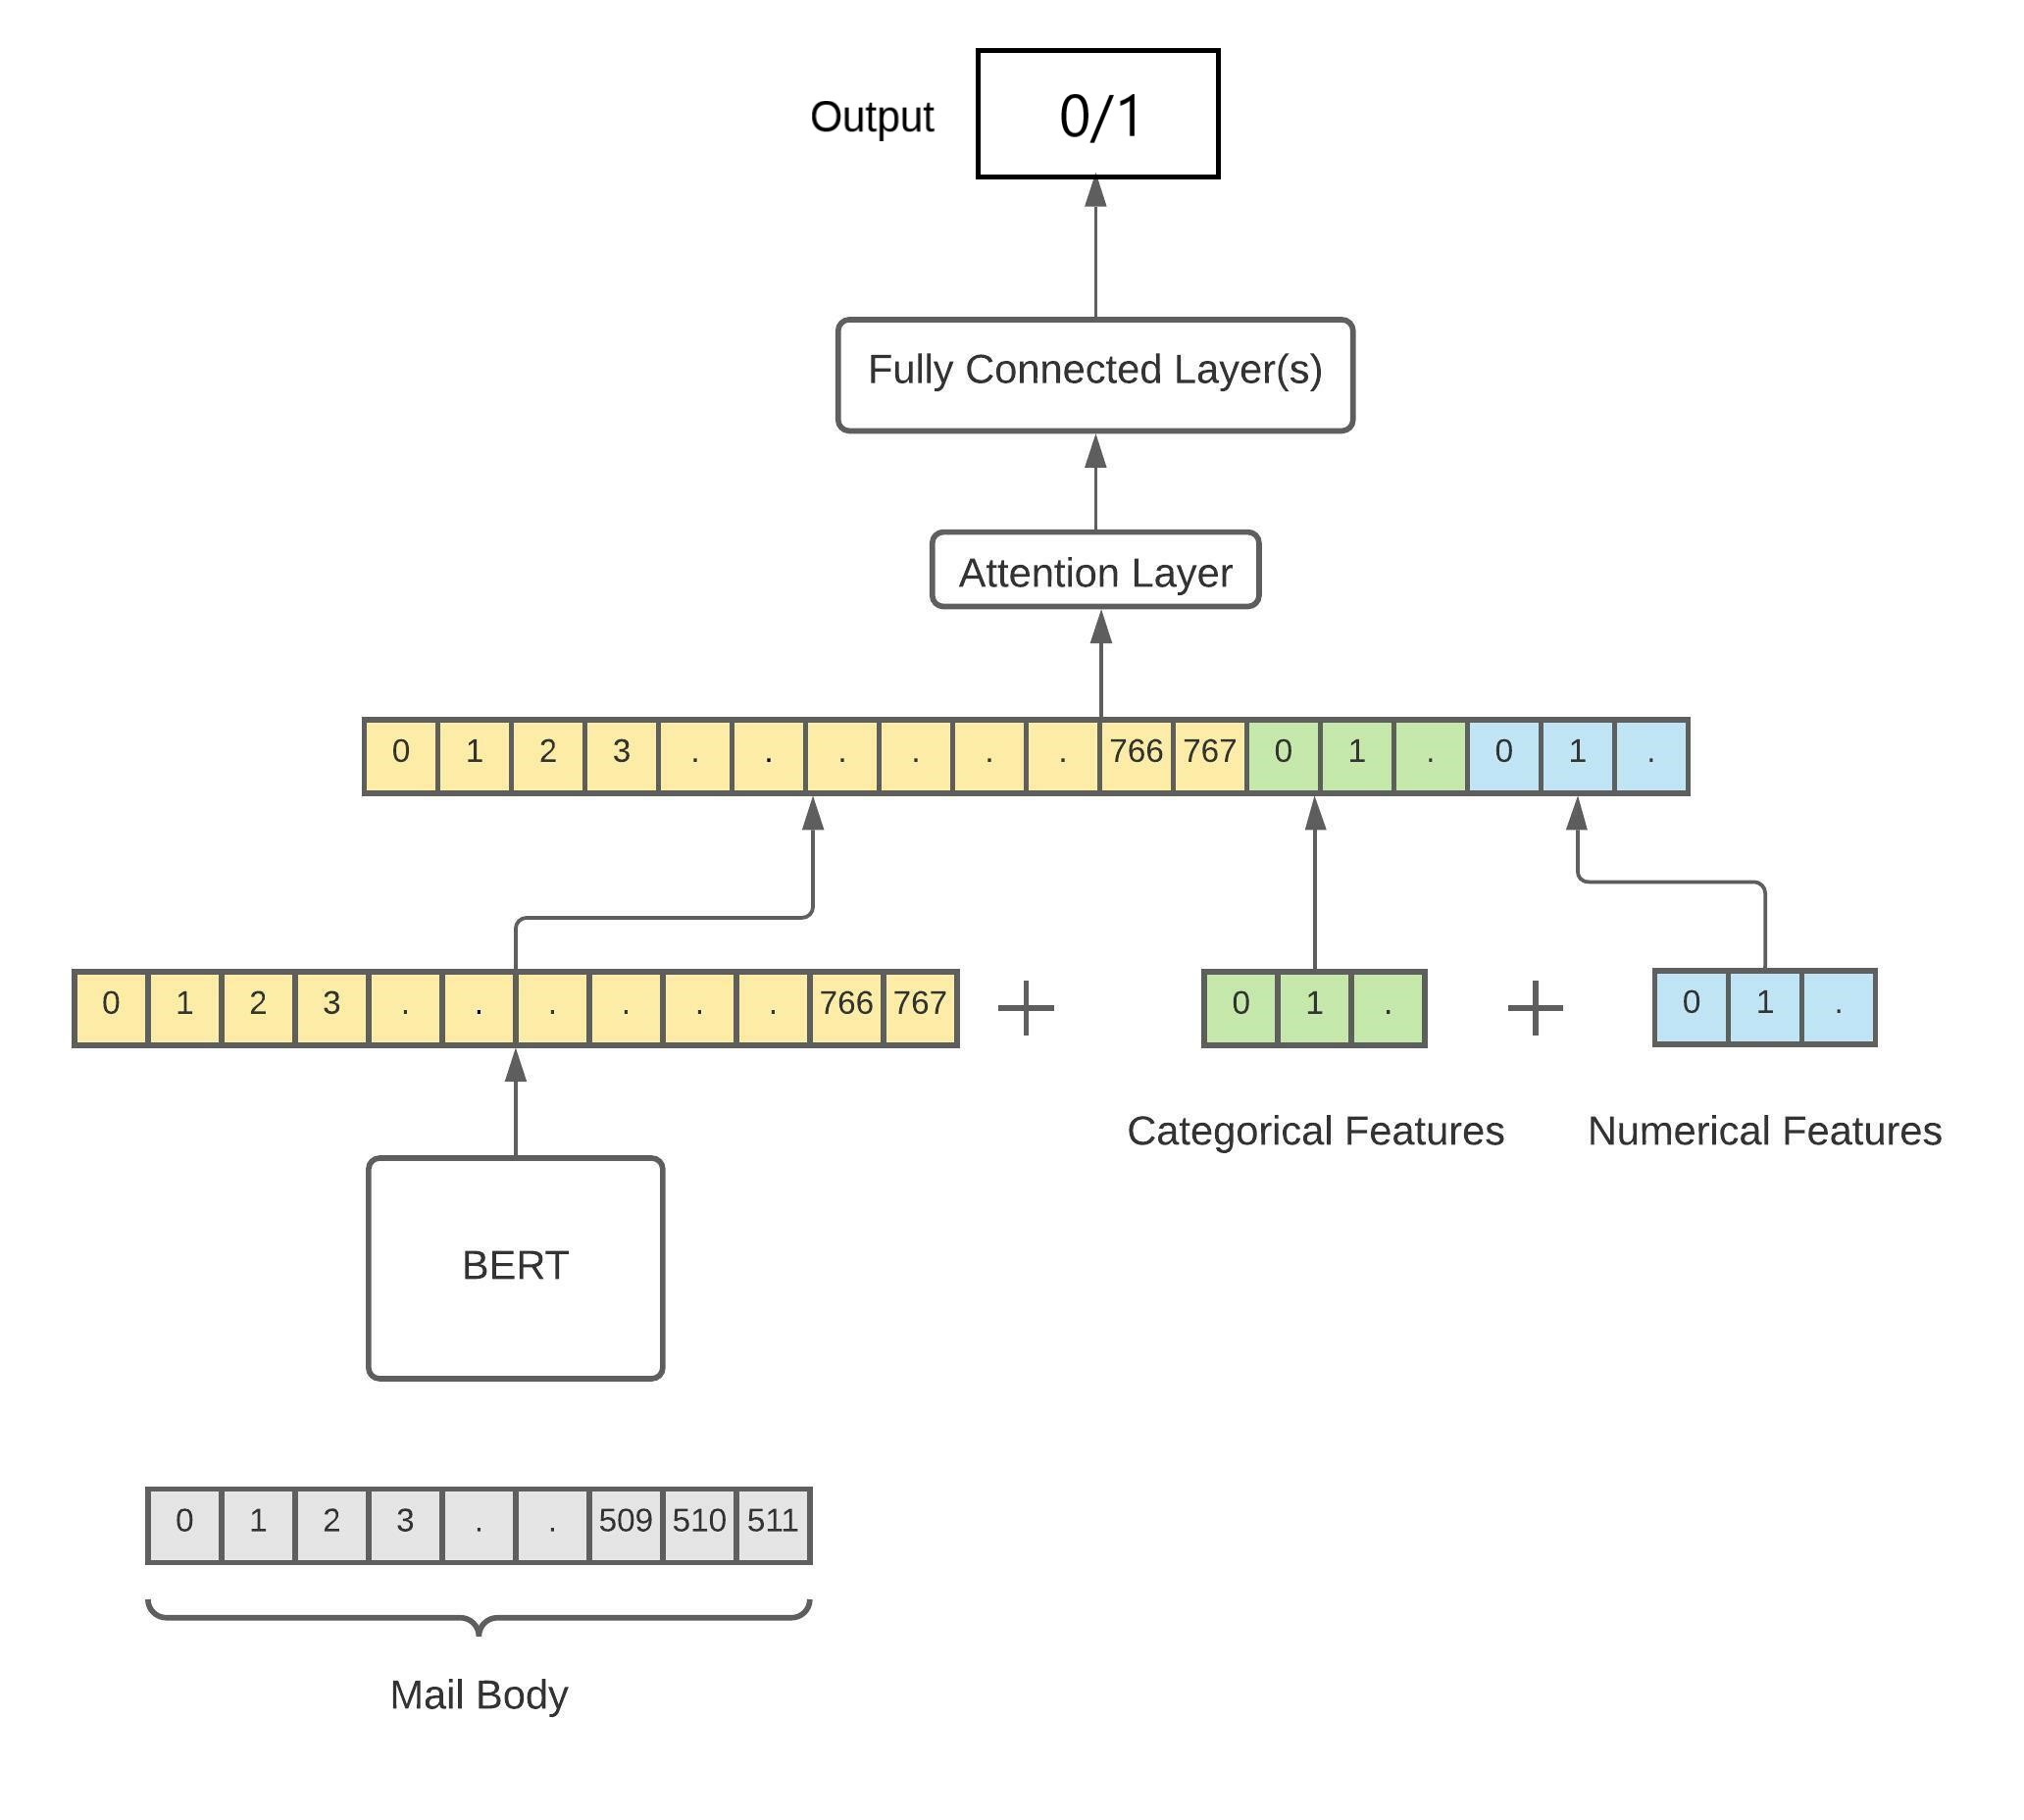
\includegraphics[scale=0.3]{Figures/model_architecture_lucid.jpg}
    \rule{10em}{0.5pt}
  \caption[Model Architecture]{Model Architecture}
  \label{fig:model_architecture}
\end{figure}

The model also conatins an attention layer between the final classifier layers and the concatenated email representation. This helps the model to focus on the features which are important when calculating the final probability.   

\section{Training Parameters}

\subsection{Baseline Models}

Experiments were conducted with various architectures, ranging from TF-IDF and CNN to BERT and RoBERTa.  Results from these models help us understand the metrics of similar models for this data and task. Table~\ref{tab:baseline_list} shows the complete list of baseline models used in the experiments.\\


\begin{table}[!h]
\captionsetup{textfont = large}
\caption{List of baseline models}
\label{tab:baseline_list}
\begin{center}
\resizebox{0.4\textwidth}{!}{

\begin{tabular}{|c|r|}
\hline
\textbf{Category}                                   & \textbf{Model}   \\ \hline \hline
Basic                                               & SVM + TF-IDF     \\ \hline \hline
\multirow{4}{*}{DL Based}                           & CNN              \\ \cline{2-2} 
                                                    & LSTM             \\ \cline{2-2} 
                                                    & BiLSTM           \\ \cline{2-2} 
                                                    & LSTM + Attention \\ \hline \hline
\multicolumn{1}{|l|}{\multirow{2}{*}{Transformers}} & BERT             \\ \cline{2-2} 
\multicolumn{1}{|l|}{}                              & RoBERTa          \\ \hline
\end{tabular}
}
\end{center}
\end{table}



All the DL-based baseline models were trained with following configuration:
\begin{fleqn}[5.4cm]
\begin{flalign*}
{&\text{Batch Size}}  = 1024\\
{&\text{Vocabulary Size}} = 2000\\
{&\text{Input Length}} = 200\\
{&\text{Word Embedding Dimension}} = 50\\
{&\text{Number of Epochs}} = 15\\
{&\text{Train : Test Split}} = 0.8:0.2
\end{flalign*}
\end{fleqn}

Apart from this, during each epoch the training data was split into training and validation set with a 0.8:0.2 split. This was done to monitor the validation loss. Early stopping was enabled which would stop the training if the validation loss did not improve for 3 consecutive epochs. 

\subsection{Transformer Models}

For BERT and RoBERTa, following training arguments were used:
\begin{fleqn}[5.4cm]
\begin{flalign*}
{&\text{Batch Size}}  = 150\\
{&\text{Input Length}} = 200\\
{&\text{Number of Epochs}} = 10\\
{&\text{Train : Test Split}} = 0.8:0.2\\
{&\text{Initial Learning Rate}} = 5e^{-5}\\
{&\text{Warmup Ratio}} = 0.07\\
{&\text{Weight Decay}} = 0.5
\end{flalign*}
\end{fleqn}

The loss function used to train all these models is Binary Cross Entropy. 
\begin{center}
$L(y,p) = -\big(y\log(p)+(1-y)\log(1-p)\big)$ = \text{Loss Function}\\
$y= \text{Actual Class}$\\
$p = \text{Predicted Class}$
\end{center}

For optimizer, ADAM optimizer\cite{DBLP:journals/corr/KingmaB14} was used for all baseline DL models and ADAM with Weight decaay was used for Transformer baseline models. 

\section{Experiments}

Experiments were conducted by varying the data size. Since the Influence features were only available for a small set of employees, the resulting dataset contains 18k rows as opposed to 600k rows for the whole dataset. Similarly, the features appended to the BERT embedding were also varied. The findings from all these variations have been listed in the next chapter.

